\documentclass[12pt, a4paper]{article}

\usepackage{amsmath}
\usepackage{bm}
\usepackage{array}
\usepackage{amsmath}
\usepackage[portuguese]{babel}
\usepackage{chngpage}
\usepackage{float}
\usepackage[a4paper, margin=2cm]{geometry}
\usepackage{graphicx}
\usepackage{hyperref}
\usepackage{listings}
\usepackage{setspace}
\usepackage{xcolor}

\lstdefinestyle{codestyle}{
    commentstyle=\color{teal},
    keywordstyle=\color{blue},
    numberstyle=\ttfamily\color{gray},
    stringstyle=\color{red},
    basicstyle=\ttfamily\footnotesize,
    breakatwhitespace=false,
    breaklines=false,
    keepspaces=true,
    numbers=none,
    showspaces=false,
    showstringspaces=false,
    showtabs=false,
    tabsize=4
}
\lstset{style=codestyle}

\title{\Huge \textbf{Computação Gráfica \\ \Large Trabalho Prático -- Fase IV}}
\date{18 de maio de 2025}
\author{Grupo 3}

\begin{document}

\begin{center}
    
\includegraphics[width=0.25\textwidth]{res/cover/EE-C.eps}
\end{center}

\chardef\_=`_
\onehalfspacing
\setlength{\parskip}{\baselineskip}
\setlength{\parindent}{0pt}
\def\arraystretch{1.5}

{\let\newpage\relax\maketitle}
\maketitle
\thispagestyle{empty}

\vspace*{\fill}

\begin{adjustwidth}{-2cm}{-2cm} % These values only need to be large enough to center the table
    \begin{center}
        \begin{tabular}{>{\centering}p{0.25\textwidth}
                        >{\centering}p{0.25\textwidth}
                        >{\centering}p{0.25\textwidth}
                        >{\centering\arraybackslash}p{0.25\textwidth}}
            
\includegraphics[width=3.5cm]{res/cover/A104437.png} &
            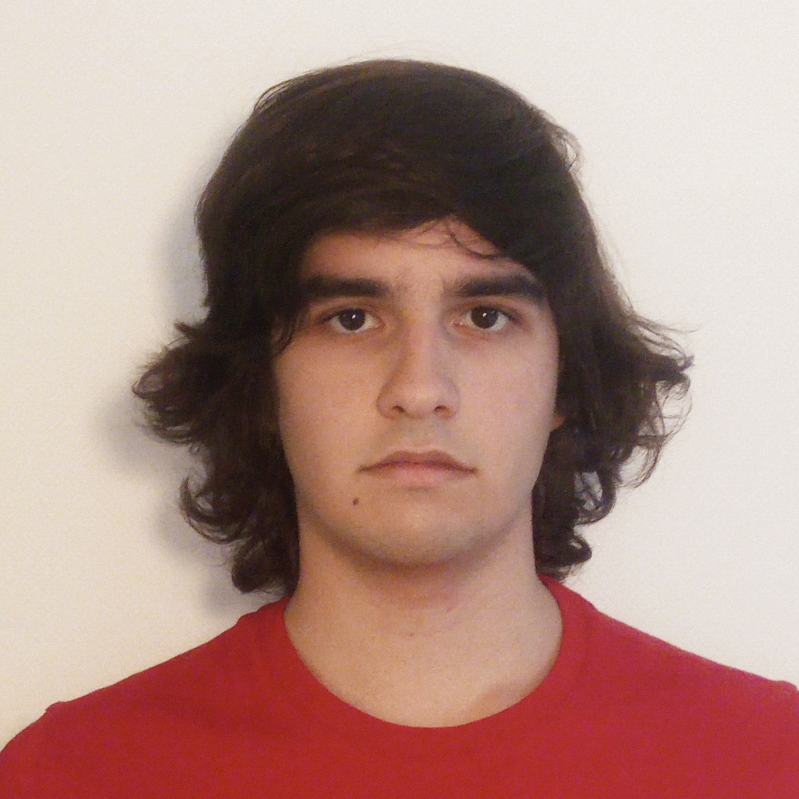
\includegraphics[width=3.5cm]{res/cover/A104348.png} &
            
\includegraphics[width=3.5cm]{res/cover/A90817.png} &
            
\includegraphics[width=3.5cm]{res/cover/A104179.png} \\

            Ana Oliveira & Humberto Gomes & Mariana Cristino & Sara Lopes \\
            A104437      & A104348        & A90817           & A104179
        \end{tabular}
    \end{center}
\end{adjustwidth}

\pagebreak

\begin{abstract}
    \noindent
    Nesta fase do trabalho prático, continuou-se o desenvolvimento dos programas \texttt{engine} e
    \texttt{generator}. Em particular, na \texttt{engine}, foram implementadas a leitura de texturas
    e a iluminação da cena. É lógico que estas funcionalidades exigiram alterações à estrutura de
    armazenamento de modelos em VBOs, ao formato XML da cena, e a criação de novos \emph{shaders},
    para implementação dos modelos de iluminação e de \emph{shading} de Phong. Adicionalmente,
    também foi implementado \emph{object picking} e geração automática de normais, para modelos que
    não têm essa informação. Do lado do \texttt{generator}, foi necessário implementar a geração de
    normais e coordenadas de textura para as figuras, bem como atualizar a geração do Sistema Solar,
    para adicionar informação de texturas e iluminação. Em suma, apesar de se considerar que o
    trabalho desenvolvido foi além do era pedido pelo enunciado, visto que foram utilizados
    \emph{shaders}, haveria muitas possibilidades de melhorar o trabalho para hipotéticas fases
    futuras (\emph{instanced rendering}, \emph{normal maps}, sombras, tesselação, \emph{etc.}).
\end{abstract}

\section{\emph{Generator}}

\subsection{Formato \texttt{.3d}}

O formato \texttt{.3d} exportado pelo \texttt{generator} e utilizado pela \texttt{engine} é o
Wavefront OBJ \cite{wavefront-obj}. Apenas uma pequena fração das funcionalidades deste formato
são suportadas e, nesta fase, foram necessárias adições aos mecanismos de escrita e leitura de
ficheiros Wavefront OBJ para suportar coordenadas de textura e normais. Este formato é textual, onde
cada linha pode ser um comentário, uma posição, uma coordenada de textura, uma normal, ou uma face
triangular, como mostra o exemplo abaixo, na ordem apresentada:

\begin{lstlisting}

# Comment
v 0.5 0.5 1
vt 0.3 0.3
vn 0 1 0
f 1/2/3 4/5/6 7/8/9
\end{lstlisting}

Quando uma linha começa com \texttt{v}, \texttt{vt} ou \texttt{vn}, devem seguir-se as coordenadas
de uma posição, de uma textura, ou de um vetor normal, respetivamente. Quando uma linha começa com
\texttt{f}, deve seguir-se uma face triangular, ou seja três pontos. O \texttt{generator} e a
\texttt{engine} suportam dois tipos de ponto:

\begin{itemize}
    \item Apenas um número, um índice de uma posição, ou seja, um elemento do tipo \texttt{v}
        (começando a contar em 1);
    \item Da forma \texttt{v/t/n}, onde estão presentes três índices, um para uma posição, um para
        uma coordenada de textura, e outro para um vetor normal.
\end{itemize}

Como o \emph{parser} de ficheiros Wavefront OBJ foi reimplementado na fase anterior com base em
expressões regulares, foi trivial adicionar o suporte para coordenadas de textura e vetores normais.

\subsection{Plano Horizontal}

{\color{red} TODO - Humberto}

\subsection{Cubo}

{\color{red} TODO - Humberto}

\subsection{Esfera}

As normais da esfera são calculadas de forma muito simples: para cada vértice, a normal é o vetor
que vai do centro da esfera até esse vértice, normalizado. Como a esfera está centrada na origem,
isso equivale a normalizar o próprio vetor posição do vértice. Este método garante que todas as
normais são perpendiculares à superfície.

As coordenadas de textura (u, v) são atribuídas com base na posição angular de cada ponto. O valor
de u varia entre 0 e 1 ao longo da longitude, e o valor de v varia entre 0 e 1 ao longo da latitude.

Nos polos, como existe apenas um vértice em cada um e é necessário ligá-lo a todas as \emph{slices}
ao redor, o mesmo vértice recebe várias coordenadas de textura com valores diferentes de u.
Isto permite ``cortar'' a textura em triângulos que convergem para os polos — como se estes fossem
divididos em pequenas fatias triangulares.
Desta forma, conseguimos aplicar uma imagem 2D na superfície da esfera de forma contínua, repartindo
a textura entre os vários triângulos sem quebras visuais visíveis.

\subsection{Cone}

No cone, as normais são definidas conforme a sua geometria:

\begin{itemize}
    \item Na base do cone, as normais são verticais e viradas para baixo: $(0, -1, 0)$.
    \item Na superfície lateral, as normais são vetores perpendiculares à superfície
    inclinada (ou seja, à geratriz do cone) e são calculadas da seguinte forma:
\[
\vec{n} = \text{normalize}(\cos(\theta), \tfrac{r}{h}, \sin(\theta))
\]
onde \( \theta \) é o ângulo da fatia atual ao redor do eixo \( y \), \( r \) é o raio da
base e \( h \) é a altura do cone.
Esta fórmula resulta em vetores normais inclinados corretamente em relação à superfície
lateral do cone.
\end{itemize}

As coordenadas de textura são atribuídas da seguinte forma:

\begin{itemize}
    \item As coordenadas da base são obtidas a partir da posição do vértice no plano XZ,
    centralizadas em $(0{,}5,\ 0{,}5)$ e normalizadas para o intervalo $[0,\ 1]$,
    permitindo o mapeamento de uma textura circular sobre a base do cone.
    \item Na lateral, o valor de $u$ varia ao longo da circunferência de acordo com o ângulo
    $\theta$ em torno do eixo $y$, sendo calculado como $u = \theta / 2\pi$. O valor de $v$
    varia com a altura, indo de $v = 0$ na base até $v = 1$ no topo, de forma proporcional à
    coordenada $y$ dos vértices, ou seja, $v = y/h$.
\end{itemize}

\subsection{Cilindro}

No cilindro, as normais são definidas conforme a sua geometria:

\begin{itemize}
    \item Na base e no topo do cilidro, as normais são verticais: $(0, -1, 0)$ e $(0, 1, 0)$,
    respetivamente.
    \item Na superfície lateral, as normais são vetores radiais no plano $XZ$, ou seja, $(x, 0, z)$
    normalizado e apontam para fora.
\end{itemize}

As coordenadas de textura são atribuídas de duas formas, dependendo do modo:

\begin{itemize}
    \item No modo simples, as coordenadas da base e do topo são calculadas a partir da posição do
    vértice no plano $XZ$, centradas em $(0.5, 0.5)$. Na lateral, o valor de $u$ varia ao longo da
    circunferência e $v$ varia com a altura.
    \item No modo \texttt{multiTextured}, aplicam-se as mesmas regras, mas os valores são ajustados
    para percorrer corretamente sobre uma imagem maior que pode conter várias secções, como base,
    lateral e topo, numa única textura.
\end{itemize}

\subsection{\emph{Torus}}

{\color{red} TODO - Sara}

\subsection{Geração de modelos com base em \emph{patches} de Bézier}

Ao gerar uma superfície de Bézier, é necessário calcular as normais e as coordenadas de textura para
cada ponto da malha.

De modo que, as normais são obtidas através do produto vetorial entre as derivadas
parciais da superfície em relação a u e v. Estas derivadas representam os vetores tangentes à
superfície em cada ponto. O produto vetorial desses vetores resulta na normal, que é posteriormente
normalizada. Este processo garante uma correta iluminação durante a renderização do modelo.

As coordenadas de textura são diretamente baseadas nos parâmetros u e v, que variam entre 0 e 1.
Assim, cada ponto da superfície fica mapeado para uma posição correspondente numa imagem de textura.

No entanto, durante o cálculo das derivadas parciais, valores como $u = 0$ ou $v = 0$ podem
originar problemas numéricos nas fronteiras da superfície. De modo que, para esses casos, são
utilizados valores ligeiramente acima de zero para garantir a estabilidade do cálculo das normais.

\subsection{Outras Figuras}

Para as restantes figuras, devido à sua complexidade e ao pouco tempo disponível para a conclusão
desta fase do trabalho prático, não foram adicionadas nem coordenadas de textura nem normais. No
entanto, a \texttt{engine} ainda é capaz de importar estes modelos e de os desenhar com iluminação,
graças a um algoritmo de geração automática de normais implementado e descrito posteriormente neste
relatório.

\subsection{Sistema Solar}

Nesta fase, a cena do sistema solar evoluiu significativamente com a introdução de iluminação,
texturas e materiais. Esses elementos contribuíram para uma representação mais fiel e
envolvente do sistema solar, aumentando consideravelmente o realismo da cena e proporcionando
uma experiência visual mais imersiva.

\begin{figure}[H]
    \centering
    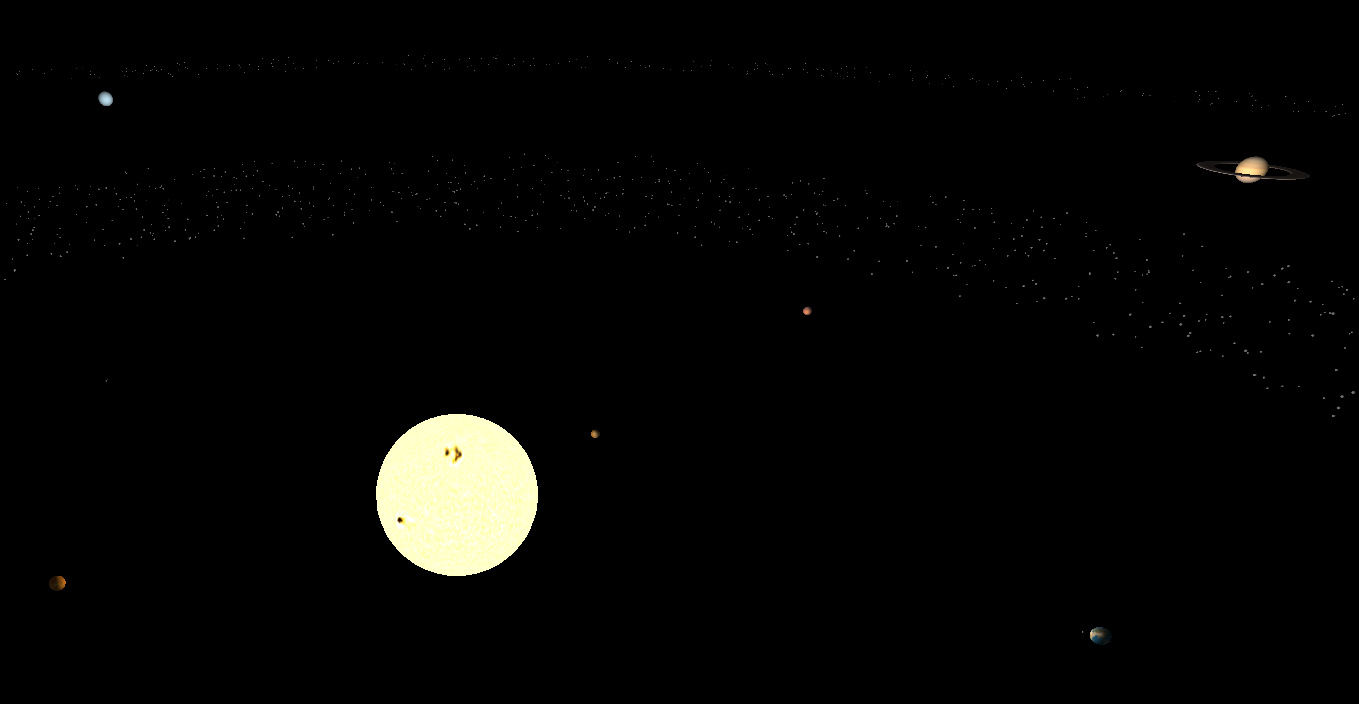
\includegraphics[width=\textwidth]{res/phase4/SolarSystem.png}
    \caption{Sistema Solar.}
\end{figure}

\section{\emph{Engine}}

\subsection{Geração Automática de Normais}

A \texttt{engine} é capaz de carregar modelos que não tenham informação sobre coordenadas de
texturas ou normais. Caso não haja informação sobre as coordenadas de textura de um modelo, é
possível desenhá-lo a uma cor sólida, mas é necessário que se tenha informação sobre as suas normais
para o iluminar corretamente. Como esta nem sempre está presente, foi implementado um algoritmo para
gerar normais de modelos automaticamente.

Este algoritmo considera o modelo inteiro como um único \emph{smoothing group}, e calcula a normal
de cada vértice como a média das normais dos triângulos a que este pertence, pesada pela área dos
triângulos. Logo, é necessário, em primeiro lugar, uma forma de calcular a normal de um triângulo.
Para um triângulo $[ABC]$, esta pode ser calculada do seguinte modo:

$$
\hat{n}_{[ABC]} = \frac{
    \overrightarrow{AB} \times \overrightarrow{AC}
}{
    \lVert \overrightarrow{AB} \times \overrightarrow{AC} \rVert
}
$$

Depois, a área de cada triângulo, $A$, pode ser calculada pela fórmula de Heron:

$$
S = \frac{
    \lVert \overrightarrow{AB} \rVert +
    \lVert \overrightarrow{AC} \rVert +
    \lVert \overrightarrow{BC} \rVert
}{
    2
}
$$

$$
A = \sqrt{
    S
    \left ( S - \lVert \overrightarrow{AB} \rVert \right )
    \left ( S - \lVert \overrightarrow{AC} \rVert \right )
    \left ( S - \lVert \overrightarrow{BC} \rVert \right )
}
$$

Logo, sendo $F$ o conjunto de faces triangulares nas quais um ponto está presente, o vetor normal
desse ponto é dado por:

$$
\hat{n} = \frac{
    \sum_{f \in F} {A_f \, \hat{n}_f}
}{
    \lVert \sum_{f \in F} {A_f \, \hat{n}_f} \rVert
}
$$

Em termos de implementação deste algoritmo, um dicionário é utilizado para armazenar associações
entre posições de pontos e pares normal-área. Iteram-se por todas as faces do modelo e, para
cada face, calcula-se a sua normal e a sua área. Depois, para cada ponto nessa face, adicionam-se
aos valores armazenados de normal e de área $A \, \hat{n}$ e $A$ respetivamente. Após iterar por
todas as faces, itera-se por todas as posições no dicionário, e define-se a normal de cada ponto
como o quociente entre a normal armazenada e a área total. Logicamente, este vetor deve ser
normalizado antes de adicionado ao modelo.

\subsection{VBOs}

Com a adição de coordenadas de textura e normais, foi necessário criar mais VBOs para as armazenar.
Agora, cada modelo passa a ter um VAO associado a três VBOs, como mostra a figura abaixo:

\begin{figure}[H]
    \centering
    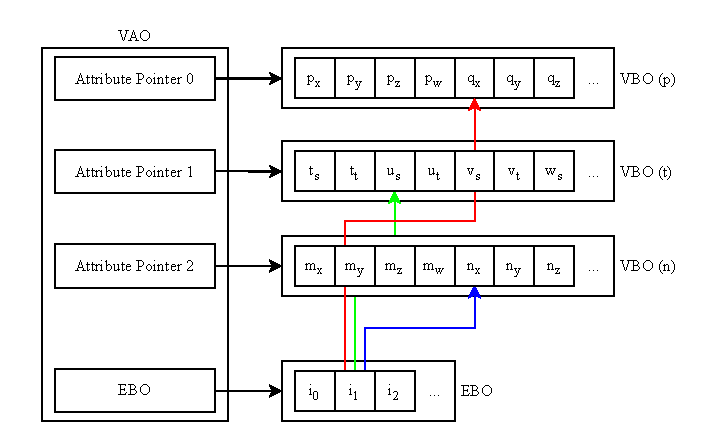
\includegraphics[width=\textwidth]{res/phase4/VAO.pdf}
    \caption{Organização do VAO, dos VBOs, e do EBO de um modelo.}
\end{figure}

Pode observar-se que, ao contrário do que acontece nos ficheiros \texttt{.3d}, não pode haver
vértices formados por posições, coordenadas de textura, e normais com diferentes índices. Para isso,
seria necessário mais do que um \emph{buffer} de índices, e isso não é suportado pelo OpenGL. Logo,
após carregar um modelo, é necessário converter o esquema de indexação de um ficheiro Wavefront OBJ
para o de um \emph{index buffer}. Para o fazer, um algoritmo simples pode ser utilizado:

\begin{itemize}
    \item Cria-se um \emph{index buffer} e três outros \emph{buffers}, para armazenamento das
        posições, das coordenadas de textura, e das normais, inicialmente vazios;

    \item Armazena-se um dicionário que associa tuplos posição-c.textura-normal a índices (elementos
        do \emph{index buffer});

    \item Iteram-se por todos os vértices no modelo. Para cada vértice:
        \begin{itemize}
            \item Constrói-se o tuplo posição-c.textura-normal associado ao vértice, que se procura
                no dicionário;
            \item Caso seja encontrado, adiciona-se o índice encontrado ao \emph{index buffer}.
            \item Caso contrário, coloca-se o tuplo no dicionário; adicionam-se a posição, a
                coordenada de textura e a normal aos seus respetivos \emph{buffers}; e adiciona-se o
                índice de um destes elementos ao \emph{index buffer}.
        \end{itemize}
\end{itemize}

\subsection{Adição ao \emph{Schema} XML}

O \emph{schema} XML foi alargado para suportar materiais com múltiplas componentes de cor, texturas
e fontes de luz diversas. Estas adições permitem um controlo mais detalhado sobre o aspeto visual
dos modelos, a aplicação de texturas e a iluminação da cena.

\subsubsection{Materiais}

Pode ser associado a cada modelo um conjunto de propriedades de material que influenciam a forma
como este interage com a luz. Estas propriedades são definidas no elemento \texttt{<color>}, onde é
possível incluir as componentes \texttt{diffuse}, \texttt{ambient}, \texttt{specular} e
\texttt{emissive}, bem como o valor de \texttt{shininess}. Caso o elemento \texttt{<color>} não
esteja presente, são utilizados valores por omissão.

\begin{lstlisting}[language=xml]
<model file="sphere.3d">
    <texture file="earth.jpg" />
    <color>
        <diffuse  R="200" G="200" B="200" />
        <ambient  R="50"  G="50"  B="50"  />
        <specular R="0"   G="0"   B="0"   />
        <emissive R="0"   G="0"   B="0"   />
        <shininess value="0" />
    </color>
</model>
\end{lstlisting}

Estas propriedades são processadas na classe \texttt{Material}, que interpreta os valores a partir
do XML através de funções auxiliares definidas no módulo \texttt{XMLUtils}. O motor de renderização
utiliza depois estes parâmetros para configurar o shader correspondente.

\subsubsection{Texturas}

Caso o elemento \texttt{<texture>} esteja presente, é carregado o ficheiro de textura especificado
e aplicado ao modelo 3D. A ausência deste elemento implica que o modelo será renderizado apenas com
base nas cores definidas no material.

\begin{lstlisting}[language=xml]
<model file="cylinder.3d">
    <texture file="metal.jpg" />
</model>
\end{lstlisting}

No carregamento da cena, o caminho da textura é resolvido com base no diretório do ficheiro XML, e
a imagem é carregada para memória. O motor assegura que a mesma textura não é carregada múltiplas
vezes, reutilizando instâncias já existentes. Esta otimização é feita através de um \texttt{map}
que armazena texturas já processadas.

\subsubsection{Iluminação}

Foi também introduzido suporte para os diferentes tipos de luzes: pontuais, direcionais e
\emph{spotlights}. Todas as fontes de luz devem ser declaradas dentro do elemento \texttt{<lights>}
no ficheiro XML da cena. Cada elemento \texttt{<light>} possui um atributo \texttt{type} e
argumentos adicionais consoante o tipo de luz especificado:

\begin{itemize}
    \item \texttt{point}: requer os atributos \texttt{posX}, \texttt{posY}, \texttt{posZ} (posição);
    \item \texttt{directional}: solicita \texttt{dirX}, \texttt{dirY}, \texttt{dirZ} (direção);
    \item \texttt{spotlight}: necessita da posição, da direção e o ângulo de corte
    (\texttt{cutoff}).
\end{itemize}

\begin{lstlisting}[language=xml]
<lights>
    <light type="point"      posX="0" posY="10" posZ="0" />
    <light type="directional" dirX="1" dirY="1" dirZ="1"/>
    <light type="spotlight"  posX="0" posY="10" posZ="0"
                             dirX="1" dirY="1" dirZ="1"
                             cutoff="45" />
</lights>
\end{lstlisting}

A criação dinâmica das instâncias de luz é realizada pela \texttt{LightFactory}, com base no
atributo \texttt{type}. Cada instância herda da interface \texttt{Light}, e é posteriormente
adicionada à lista de luzes da cena.

\subsection{Texturas e Iluminação}

O principal objetivo desta fase do trabalho prático é a adição de texturas e iluminação ao projeto.
Com a informação de coordenadas de textura e normais nos modelos, e informação sobre luzes,
materiais, e caminhos para imagens nos ficheiros de cena, é agora possível que a \texttt{engine}
desenhe os objetos de uma cena iluminados e com texturas.

Para carregar as texturas para a memória, a biblioteca \texttt{stb\_image} \cite{stb-image} é
utilizada. Como o referencial de coordenadas de textura em OpenGL tem a sua origem no canto inferior
esquerdo, mas o referencial regularmente utilizado em imagens tem a sua origem no canto superior
esquerdo, a função \texttt{stbi\_set\_flip\_vertically\_on\_load} é utilizada para inverter
verticalmente todas as imagens lidas. Depois de carregar uma imagem, é possível criar uma textura,
vinculá-la, definir os seus parâmetros de \emph{wrapping} e \emph{filtering}, enviar os dados da
textura para a GPU, gerar \emph{mipmaps}, e libertar a memória ocupada pela imagem inicialmente
carregada. Tal como é feito para o carregamento de modelos, caso uma cena referencie a mesma imagem
mais do que uma vez, apenas uma textura será criada, assim poupando memória da GPU.

Para desenhar os objetos da cena com texturas e iluminação, foi necessário criar novos
\emph{shaders} para o efeito. Como alguns objetos na cena não são iluminados (eixos, linhas de
animação, esferas encapsuladoras, \emph{etc.}), é necessário trocar de programa sempre que se deseja
desenhar um destes objetos. Para minimizar o número de trocas de programa, uma operação com um custo
elevado para o desempenho, todos os objetos não iluminados são desenhados em primeiro lugar, e só
depois se renderizam os restantes.

Ao contrário da \emph{fixed-function pipeline} do OpenGL, que implementa \emph{shading} de Gouraud,
os \emph{shaders} desenvolvidos utilizam \emph{shading} de Phong, onde as equações da luz são
computadas para cada fragmento, com base em normais interpoladas pelo \emph{shader} de vértices.
Assim, as manchas especulares são representadas muito mais claramente do que seriam caso a
\emph{fixed-function pipeline} tivesse sido utilizada. Ademais, devido ao uso de \emph{shaders}, é
possível ter mais do que oito luzes numa cena, o número exigido pelo enunciado. Agora, o limite
máximo de luzes é ditado pelo número máximo de variáveis uniformes num programa, que depende do
\emph{hardware} utilizado.

Antes de apresentar os \emph{shaders} desenvolvidos, é necessário apresentar alguma notação para as
matrizes utilizadas:

\begin{itemize}
    \item $P$ - Matriz de projeção, que converte coordenadas do espaço da câmara para
        \emph{clip-space};
    \item $V$ - Matriz de vista, que converte coordenadas do espaço do mundo para o espaço da
        câmara;
    \item $M$ - Matriz do modelo, que converte coordenadas do espaço local (do modelo) para o espaço
        do mundo;
\end{itemize}

Comece-se por perceber o funcionamento do \emph{shader} de vértices. Este, como o outro
\emph{shader} previamente desenvolvido, também multiplica as coordenadas dos pontos do modelo a
desenhar pela matriz $PVM$ (passada ao \emph{shader} numa variável uniforme), colocando-as em
\emph{clip-space} antes de serem passadas ao \emph{shader} de fragmentos. No entanto, agora também é
necessário tratamento das coordenadas de texturas e das normais. As coordenadas de textura são
passadas ao \emph{shader} de fragmentos sem qualquer transformação (apenas interpolação). As
normais, para continuarem perpendiculares às superfícies a que se referem, mesmo após a aplicação de
escalas não uniformes, são multiplicadas pela matriz $(M^T)^{-1}$ \cite{learn-opengl-1}, também
passada ao \emph{shader} numa variável uniforme. Isto converte-as para o espaço do mundo, onde os
cálculos das equações da luz serão feitos
\footnote{Apesar de, para o cálculo das equações da
luz ser feito no espaço do mundo, ser necessária mais uma variável uniforme (a posição da câmara),
achámos este método um pouco mais intuitivo e fácil de depurar do que fazer os mesmo cálculos no
espaço da câmara.}.
Em último lugar, é calculada e passada ao \emph{shader} de fragmentos (após uma interpolação) a
posição do vértice no espaço do mundo, ou seja, a posição do vértice do modelo multiplicada pela
matriz $M$, passada ao \emph{shader} de vértices numa variável uniforme.

O \emph{shader} de fragmentos, antes de poder calcular a cor de qualquer ponto, deve, em primeiro
lugar, renormalizar o vetor normal que recebe interpolado do \emph{shader} de fragmentos, visto que
o seu comprimento pode diminuir durante a interpolação. Desta operação resulta o vetor que se
denominará $\hat{n}$. Ademais, também é necessário calcular a direção do fragmento para a câmara,
$\hat{e}$, dada pela diferença entre a posição da câmara e a posição do fragmento, seguida de uma
normalização.

Para cada luz, é necessário calcular o vetor normalizado que aponta para a luz, $\hat{l}$. Para as
luzes direcionais, este valor é constante e passado ao \emph{shader} por uma variável uniforme. Para
as \emph{point lights} e \emph{spotlights}, este vetor é a diferença entre a posição da luz e a
posição do fragmento, seguido de uma normalização.

De um modo geral, o contributo da $i$-ésima luz para a componente difusa da cor de um fragmento,
$D_i$ é dado pela seguinte expressão \cite{learn-opengl-1}, onde $K_d$ representa a componente
difusa do material aplicado ao objeto:

$$
D_i = K_d \times \max \left ( 0, \cos \left ( \angle (\hat{n}, \hat{l}) \right ) \right )
$$

Como os vetores $\hat{n}$ e $\hat{l}$ se encontram normalizados, e tendo em conta que
$
\vec{u} \, \cdot \, \vec{v} =
\lVert \vec{u} \rVert \, \lVert \vec{v} \rVert \cos (\angle (\vec{u}, \vec{v}))
$
é possível simplificar a expressão acima do seguinte modo:

$$
D_i = K_d \times \max \left ( 0, \hat{n} \cdot \hat{l} \right )
$$

O contributo da $i$-ésima luz para a componente especular da cor do fragmento, $S_i$, é calculado
de acordo com a seguinte expressão, onde $K_s$ e $s$ representam a componente especular e o fator
\emph{shininess} do material aplicado ao objecto, respetivamente:

$$
S_i = K_s \times \left ( \max \left (0, \hat{e} \cdot \hat{r} \right ) \right ) ^ s
$$

Na expressão acima, $\hat{r}$ representa o raio da luz refletido, calculado pela função
\texttt{reflect} do GLSL.

Em relação à diferença entre os vários tipos de luz, já se explicou que é necessário calcular a
direção da luz para as \emph{point lights} e \emph{spotlights}. Em relação a estas luzes, não se
implementou qualquer forma de atenuação, visto que o formato XML da cena não permite a sua definição
e, por omissão, em OpenGL as luzes não sofrem qualquer atenuação \cite{glLight}. Também pelo mesmo
motivo, nas expressões apresentadas acima, a intensidade da luz não é considerada, visto que esta é
a mesma para em todas as luzes, 1. No entanto, é necessário algum cuidado com as \emph{spotlights}.
Para o contributo de uma destas luzes não ser nulo, é necessário que o fragmento esteja dentro do
cone de luz, ou seja, que o ângulo entre o raio de luz e o simétrico do vetor de direção da
\emph{spotlight} seja inferior ao \emph{cutoff} $\theta$ \cite{learn-opengl-2}:

\begin{align*}
    & \angle (\hat{l}, -\hat{d}) \le \theta \\
    \Leftrightarrow & \cos \left ( \angle (\hat{l}, -\hat{d}) \right ) \le \cos \theta \\
    \Leftrightarrow & \, \hat{l} \cdot (-\hat{d}) \le \cos \theta
\end{align*}

Na prática, o cosseno do ângulo de \emph{cutoff} de uma \emph{spotlight} é passado ao \emph{shader}
numa variável uniforme, e o \emph{shader} faz a comparação acima para verificar se um fragmento é
ou não iluminado por essa \emph{spotlight}.

Estando calculadas as contribuições de todas as luzes, a cor de um fragmento pode ser determinada do
seguinte modo, onde $K_a$ e $K_e$ representam a componentes ambiente e emissiva do material aplicado
ao objeto, respetivamente \cite{learn-opengl-1} \cite{learn-opengl-3}:

$$
K = K_a + K_e + \sum_{i} D_i + \sum_{i} S_i
$$

Quando um objeto é desenhado com uma textura, a cor amostrada da textura é utilizada, nas
expressões acima, como a componente difusa do material, e a componente ambiente é uma fração da cor
da textura (por omissão, um quinto).

Abaixo, segue-se um diagrama a explicar como estes \emph{shaders} desenvolvidos se encaixam na
\emph{pipeline} de renderização:

\begin{figure}[H]
    \centering
    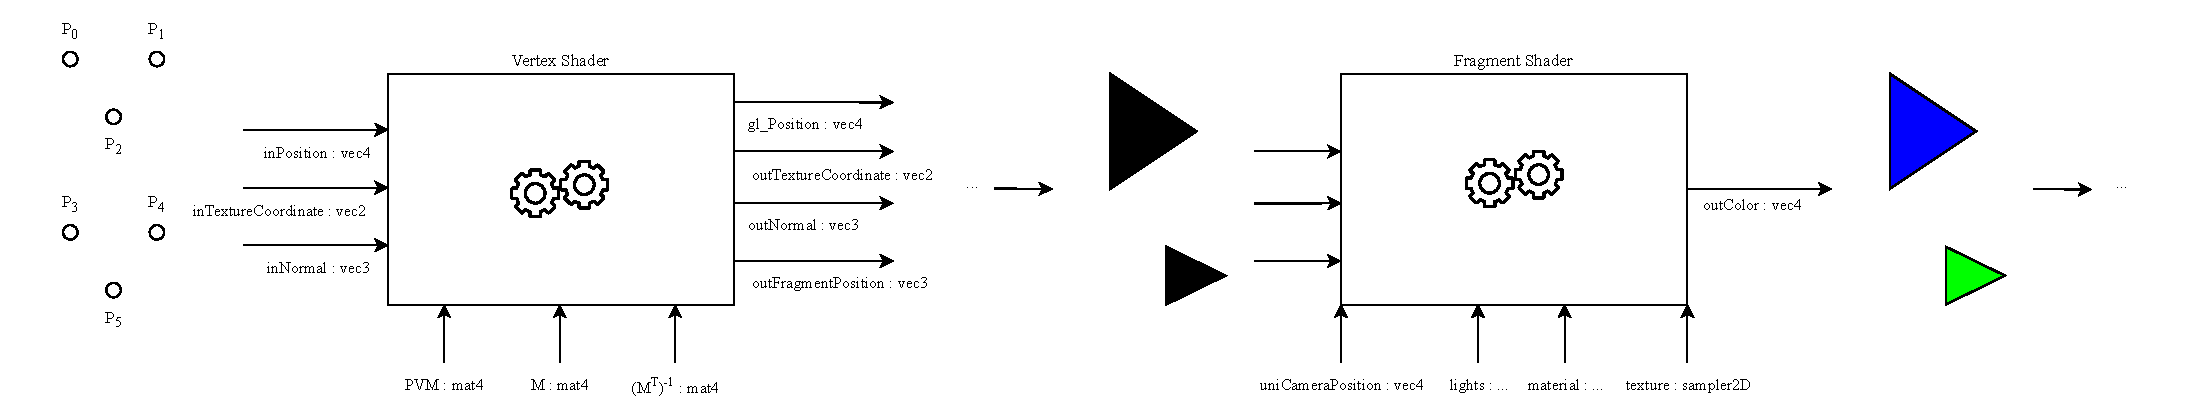
\includegraphics[width=\textwidth]{res/phase4/Shaders.pdf}
    \caption{Esquema dos \emph{shaders} desenvolvidos na \emph{pipeline} de renderização.}
\end{figure}

\subsection{\emph{Object Picking}}

{\color{red} TODO - Sara}

\section{Resultados Obtidos}

{\color{red} TODO - cada faz as suas prints, sem borda de janela, no tamanho especificado pela cena,
com a UI escondida (U), Humberto escreve}

\begin{figure}[H]
    \centering
    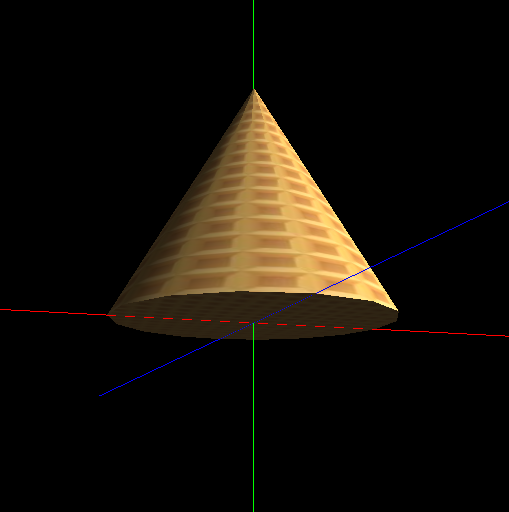
\includegraphics[width=\textwidth]{res/phase4/Cone.png}
    \caption{Cone.}
\end{figure}

\begin{figure}[H]
    \centering
    
\includegraphics[width=\textwidth]{res/phase4/IceCream.png}
    \caption{Gelado.}
\end{figure}

\begin{figure}[H]
    \centering
    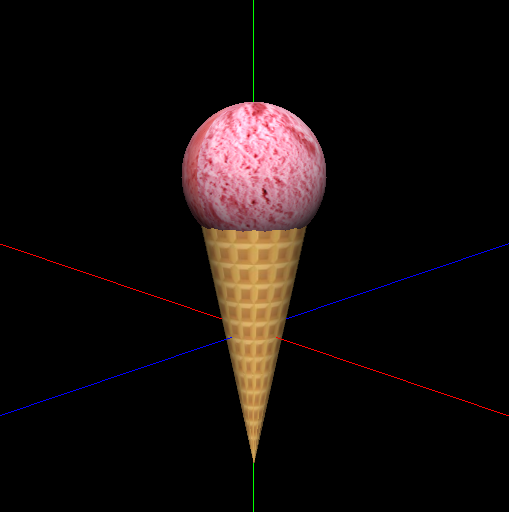
\includegraphics[width=\textwidth]{res/phase4/IceCreamXYZ.png}
    \caption{Gelado.}
\end{figure}

\section{Conclusão}

Em suma, considera-se que a quarta fase do trabalho prático foi concluída com sucesso. Apesar desta
fase ter sido a mais exigente, requirindo alterações a diversas partes da \texttt{engine} e do
\texttt{generator}, o nosso grupo foi capaz de utilizar todo o conhecimento que tem vindo a adquirir
ao longo do último semestre para implementar todas as funcionalidades pedidas, e ainda algumas
adicionais! Também foi uma grande ajuda a reestruturação arquitetural do código feita na 3.ª fase,
que tornou mais simples a adição de novas funcionalidades.

As maiores dificuldades sentidas nesta fase deram-se no \texttt{generator}, no que toca à adição de
coordenadas de texturas e normais, tendo sido difícil garantir que todas as figuras tinham um aspeto
correto, e descobrir a origem dos erros que se iam encontrado: coordenadas de texturas erradas
\emph{vs.} distorção natural inevitável, ou normais erradas \emph{vs.} implementação incorreta da
iluminação.

Em relação às funcionalidades previstas na 3.ª fase, \emph{object picking} foi implementado, mas não
houve tempo para implementar \emph{instanced rendering}. No entanto, para as cenas desenvolvidas, a
falta desta funcionalidade não se provou um problema, visto que o elemento do grupo com a placa
gráfica menos capaz (Intel HD Graphics 630), conseguia correr à taxa de atualização do seu ecrã
(60Hz) a cena mais complexa, o Sistema Solar, que pode exigir milhares de \emph{draw calls}.

Conclui-se este trabalho com grande satisfação em relação ao resultado final, que se considera
cumprir as funcionalidades pedidas pelo enunciado, bem como implementar muitas outras. No entanto,
um possível ponto que poderia ser melhorado seria o subsistema de câmaras, que tem em
falta aceleração e desaceleração suaves quando perante \emph{input} do utilizador. Apesar desta ser
a última fase do trabalho prático, há muitas funcionalidades que poderiam ser implementadas caso
houvesse tempo para tal em hipotéticas futuras fases, desde aspetos simples como uma \emph{skybox} e
LODs, como outros mais complexas apenas possíveis por se ter arquiteturado o projeto para usar
\emph{shaders}, como sombras, reflexões, \emph{normals maps}, tesselação, \emph{physically based
rendering}, \emph{etc.}.

\begingroup
\section{Bibliografia}
\renewcommand{\section}[2]{}

\begin{thebibliography}{9}
    \bibitem{wavefront-obj}
        ``Wavefront OBJ File Format Summary.''{} FileFormat.Info. Accessed: May 14, 2025. [Online.]
        Available: \url{https://www.fileformat.info/format/wavefrontobj/egff.htm}
    \bibitem{stb-image}
        ``stb.'' GitHub. Accessed: May 13, 2025. [Online.] Available:
        \url{https://github.com/nothings/stb}
    \bibitem{learn-opengl-1}
        ``Basic Lighting.'' Learn OpenGL. Accessed: May 13, 2025. [Online.] Available:
        \url{https://learnopengl.com/Lighting/Basic-Lighting}
    \bibitem{glLight}
        ``glLight''. Khronos Registry. Accessed: May 13, 2025. [Online.] Available:
        \url{https://registry.khronos.org/OpenGL-Refpages/gl2.1/xhtml/glLight.xml}
    \bibitem{learn-opengl-2}
        ``Light casters.'' Learn OpenGL. Accessed: May 13, 2025. [Online.] Available:
        \url{https://learnopengl.com/Lighting/Light-casters}
    \bibitem{learn-opengl-3}
        ``Multiple Lights.'' Learn OpenGL. Accessed: May 13, 2025. [Online.] Available:
        \url{https://learnopengl.com/Lighting/Multiple-lights}
\end{thebibliography}
\endgroup

\end{document}
